\documentclass{llncs}
\usepackage{graphicx, subfigure, amsmath, xspace, txfonts}

\begin{document}
\newcommand{\comment}[1]{}

\author{Jan David Mol, John W. Romein and Rob V. van Nieuwpoort}
\title{The LOFAR Beamformer: \\ Implementation and Performance Analysis}
\institute{Stichting ASTRON (Netherlands Institute for Radio Astronomy) \\ Oude Hoogeveensedijk 4, 7991 PD Dwingeloo, The Netherlands \\ \texttt{\{mol,romein,nieuwpoort\}@astron.nl}}
\maketitle


\begin{abstract}
Traditional radio telescopes use one or several large steel dishes to observe a single source. The LOFAR telescope is different and features a novel design in several ways. It uses tens of thousands of fixed omnidirectional antennas, the signals of which are centrally combined in real time. The LOFAR telescope focusses on a source by performing a weighted addition of the signal streams originating from groups of antennas (stations). We can focus our telescope in multiple directions in parallel by combining the signal streams from the stations multiple times using different weights. In fact, the parallel processing power and high-speed interconnect in our supercomputer allows us to look at hundreds of sources at the same time. The power to observe many sources in parallel serves a broad range of scientific astronomical interests, and creates novel opportunities for performing astronomical observations.

LOFAR is also the first major telescope to process its data in software, instead of needing a dedicated hardware design. By using software, the processing remains flexible and scalable, and new features are easier to implement and to maintain. It is through the use of software that we can fully explore the novel features and the power of our unique instrument.

In this paper, we present the processing pipeline in our supercomputer which enables our parallel observations. Our so-called \emph{Pulsar Pipeline}, named after the use case that pushed its development, is implemented on a supercomputer, and receives up to 64 data streams from the stations at 3.1 Gb/s each. Inside the supercomputer, signal-processing techniques and two all-to-all exchanges are performed. Our pulsar pipeline further expresses the power of a software telescope implemented using parallel processing techniques. We present the trade-offs in our design, the CPU and I/O performance bottlenecks that we encounter, as well as the scaling characteristics and its real-time behaviour. 
      
\comment{
  
}
\end{abstract}
\section{Introduction}

\comment{
  EUROPAR 2011:
    - abstract 24 jan
    - deadline 31 jan
    - 12 pagina's LNCS, incl broncode
}

\comment{
lofar:
  - overview
  - #stations
  - data rates

pulsar pipeline:  
  - new astronomical opportunities:
        - dynamic focus -> hundreds of simultaenous observations, which regular dishes must do sequentially
        - broad sky view -> surveys
        - extremely high data rates (up to 200 Gbit/s in, 18 Gbit/s out)
                - disks limits output rate, to be raised to 80Gbit/s out.

==> power of parallel machines + flexibility of software = powerful telescope                

software correlator benefits:
  the- flexibility
  - fast rollout of experimental features
  - easy bugfixing
  - high level programming -> advanced and complex features

}

The LOFAR (LOw Frequency ARray) telescope is the first of a new generation of radio telescopes. Instead of using a set of large, expensive dishes, LOFAR uses many thousands of simple antennas. Every antenna observes the full sky, and the telescope can be aimed through signal processing techniques. LOFAR's novel design allows the telescope to perform wide-angle observations as well as to observe in multiple directions simultaneously, neither of which are possible when using traditional dishes. In several ways, LOFAR will be the largest telescope in the world, and will enable ground-breaking research in several areas of astronomy and particle physics~\cite{Bruyn:02}.

Another novelty is the elaborate use of software to process the telescope data in real time. Previous generations of telescopes depended on custom-made hardware to combine data, because of the high data rates and processing requirements. The availability of sufficiently powerful supercomputers however, allow the use of software to combine telescope data, creating a more flexible and reconfigurable instrument.

For processing LOFAR data, we use an IBM BlueGene/P (BG/P) supercomputer. The LOFAR antennas are grouped into stations, and each station sends its data (up to 200 Gb/s for all stations) to the BG/P super computer. Inside the BG/P, the data are split and recombined using both real-time signal processing routines as well as two all-to-all exchanges. The output data streams are sufficiently reduced in size in order to be able to stream them out of the BG/P and store them on disks in our storage cluster.

The stations can be configured to observe in several directions in parallel, but have to divide their output bandwidth among them. In this paper, we present the \emph{pulsar pipeline}, an extension to the LOFAR software which allows the telescope to be aimed in tens of directions simultaneously at LOFAR's full observational bandwidth, and in hundreds of directions at reduced bandwidth. Both feats cannot be matched by any other telescope. The data streams corresponding to each observational direction, called \emph{beams}, are generated through (weighted) summations of the station inputs, which are demultiplexed using an all-to-all exchange, and routed to the storage cluster.

Using the pulsar pipeline, astronomers can focus on known pulsars, planets, exoplanets, the sun, and other objects, with unprecedented sensitivity. Furthermore, our pipeline allows fast broad-sky surveys to discover new pulsars, by observing in hundreds of directions in parallel. 

% TODO: mention other uses / observation types

In this paper, we will show how a software solution and the use of massive parallellism allows us to achieve this feat. We provide an in-depth study on all performance aspects, real-time behaviour, and scaling characteristics. The paper is organised as follows.

\section{Related Work}

MWA.

LOFAR imaging pipeline \cite{Romein:10a}

\section{LOFAR}
\label{Sec:LOFAR}

The LOFAR telescope consists of many thousands of simple dipole antennas (see Figure \ref{fig:lbafield}), grouped in \emph{stations}. The stations are strategically placed, with six stations acting as its center (the \emph{core}) and TODO stations at increasing distances from that core. Every station collects and combines the signals from its antennas, and sends the resulting data stream to our IBM BlueGene/P (BG/P) supercomputer at our central processing facility. The BG/P combines the data streams from one or more stations and reduces the resulting stream in size sufficiently to be able to store it on disks in our storage cluster. Both the stations and the BG/P perform hard-real-time signal processing. Once the data has been stored on disk, off-line processing takes over. The off-line processing transforms and further reduces the data produced by the BG/P into data products such as images or time series, and are made available to the astronomer(s) that requested the observation.

\begin{figure}[ht]
\subfigure[A field with low-band antennas (dipoles).]{
  \makebox[60mm][c]{
     \includegraphics[width=0.4\textwidth]{LBA-field.jpg}
     \label{fig:lbafield}
  }
}
\hfill
\subfigure[The left antenna receives the wave later.]{
  \makebox[50mm][c]{
    \includegraphics[width=0.4\textwidth]{delay.pdf}
    \label{fig:delay}
  }
}
\caption{LOFAR antennas}
\end{figure}

The antennas are omnidirectional and have no moving parts. Instead, all telescope functions are performed electronically through signal processing done at the stations and on the BG/P. The telescope can be aimed because the speed of light is finite: the light emitted by a source will arrive at different antennas at different times (see Figure \ref{fig:delay}). By adding appropriate delays to the signals from individual antennas before accumulating them, the signals from the source will be amplified with respect to signals from other directions. Once the samples from all antennas are combined, the data are transmitted to the BG/P, which uses the same technique to combine the data from the individual stations. The latter will be explained further in Section \ref{Sec:Beamforming}.

A LOFAR station is able to produce 248 frequency subbands of 195~kHz out of the sensitivity range of 80~MHz to 250~MHz. Each sample consists of two complex 16-bit integers, representing the amplitude and phase of the X and Y polarizations of the antennas. The resulting data stream from a station is a 3.1~Gb/s UDP stream.

\comment{
  Hardware:
    - stations and antennas
    - network

  Processing in general:
    - station processing
        - how aiming works
    - online processing
    - offline processing
}

\section{IBM BlueGene/P}

We use an IBM BlueGene/P (BG/P) supercomputer for the real-time processing of station data. We will describe the key features of the BG/P, but more information can be found elsewhere~\cite{IBM:08}. Furthermore, we will describe how our BG/P is connected to its input and output systems.

\subsection{System Description}

Our system consists of 3 racks, with 12,480 processor cores that provide 42.4 TFLOPS peak processing power. One chip contains four PowerPC~450 cores, running at a modest 850~Mhz clock speed to reduce power consumption and to increase package density. Each core has two floating-point units (FPUs) that provide support for operations on complex numbers. The chips are organised in \emph{psets}, each of which consists of 64 cores for computation (\emph{compute cores}) and one chip for communication (\emph{I/O node}). Each compute core runs a fast, simple, single-process kernel (the Compute Node Kernel, or CNK), and has access to 512 MiB of memory. The I/O nodes consist of the same hardware as the compute nodes, but additionally have a 10~Gb/s Ethernet interface connected. Also, they run Linux, which allows the I/O nodes to do full multitasking. One rack contains 64 psets, which is equal to 4096 compute cores and 64 I/O nodes.

The BG/P contains several networks. A fast \emph{3-dimensional torus\/} connects all compute nodes and is used for point-to-point and all-to-all communications. The torus uses DMA to offload the CPUs and allows asynchronous communication. The \emph{collective network\/} is used for MPI collective operations, but also for external communication. External communication is routed within each pset, through its I/O node using a tree configuration. The I/O node is capable of transporting 6.8~Gb/s bidirectionally to and from one or more compute nodes. Additional networks exist for fast barriers, initialization, diagnostics, and debugging. % TODO: add cross-section/link bandwidth for 3D torus?

\subsection{External Connections}

\begin{figure}[ht]
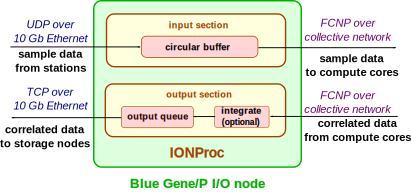
\includegraphics[width=\textwidth]{ION-processing.pdf}
\caption{Data flow diagram for the I/O nodes.}
\label{fig:ion-processing}
\end{figure}

We run a multi-threaded program on each I/O~node which is responsible for two tasks: the handling of input, and the handling of output (see Figure \ref{fig:ion-processing}). Even though the I/O nodes each have a 10~Gb/s Ethernet interface, they do not have enough computation power to handle 10~Gb/s of data. The overhead of handling IRQs, IP, and UDP/TCP put such a high load on the 850~MHz cores of the I/O nodes, that the performance seems limited to a total data rate of roughly 4~Gb/s. To achieve these data rates, we installed our own software on the I/O nodes, augmenting IBM's software stack~\cite{Yoshii:10}, and we implemented a low-overhead communication protocol called FCNP~\cite{Romein:09a} to efficiently transport data to and from the compute nodes. Recall that at full observational bandwidth, a station produces 3.1~Gb/s of data. Each I/O node can thus receive data from at most one station. The I/O nodes forward the station data to the compute nodes. The compute nodes convert the (complex) integer samples to the (complex) float domain, and perform all of the necessary on-line signal processing.

Once the compute nodes have finished processing the data, the results are sent back to the I/O nodes. The I/O nodes forward these results to our 24-node storage cluster. Each I/O node can send up to 1.1~Gb/s if it receives station data at the same time, and up to 3.1~Gb/s if the I/O node is not receiving station data. The storage cluster itself can handle up to 80~Gb/s of sustained throughput. The output queue which is maintained at the I/O node for all data uses a best-effort policy and drops data if it cannot be sent, in order to keep the BG/P running at real time.

\comment{
  BG/P explanation:
    - basic architecture and size of our installation
    - IO nodes and compute nodes
    - internal networks
    - external networks and storage nodes
}

\section{Beamforming}
\label{Sec:Beamforming}

As mentioned in Section \ref{Sec:LOFAR}, a LOFAR station is aimed at a source by applying different delays to the signals from the antennas, and subsequently adding the delayed signals. This process is known as \emph{beamforming}, which is performed at several stages in our processing pipeline. The station beamformer is implemented in hardware, in which the signal is delayed by switching it over wires of different lengths. The signals from the different antennas are subsequently added using an FPGA. The resulting beam, even though it is aimed at a certain source, is nevertheless still sensitive to signals from a large area around the source.

The BG/P, in which the signals from all the LOFAR stations come together, again performs beamforming by adding the appropriate delays to the signals from the various stations, this time in software. Because the beam produced by each station has a large sensitive area around the source, the BG/P beamformer can not only aim at the source for which the stations are configured, but also at sources around it. Different beams can then be created by adding the signals from the individual stations over and over again, each time using different delays. The delay that has to be applied depends on the relative positions of the stations and the relative direction of the beam with respect to the source. The delays are applied in software in two phases. First, the streams are aligned by shifting them a whole number of samples with respect to each other, which resolves delay differences up to the granularity of a single sample. Then, the remaining sub-sample delays are compensated for by shifting the phase of the signal. Even though a phase correction is not a proper shift because information does not shift between one sample and the next, it proves to be a good enough approximation.

This approximation is in fact good enough to limit the generation of different beams through phase corrections alone. The samples coming from different stations are shifted the same amount for all beams that are created. Because a phase shift can be performed using a complex multiplication, the beam former in the BG/P only has to accumulate the weighted vectors of samples from each station. Let $\overrightarrow{S_i}$ be the stream of samples from station $i$, $\overrightarrow{B_j}$ the stream of samples of beam $j$, and $w_{ij}$ the phase correction to be applied on station $i$ to represent the required delay for beam $j$. Then, the beam former performs the following calculation on the samples of both the X and Y polarisations independently, to obtain beam $j$:
\begin{eqnarray}
\overrightarrow{B_j} & = & \sum_{i \in \textrm{stations}}w_{ij}\overrightarrow{S_i}.
\end{eqnarray}

A beam $\overrightarrow{B_j}$ formed at the BG/P consists of a stream of complex 32-bit floating point numbers, two for each time sample (representing the X and Y polarisations), which is equal to 6.2~Gb/s at LOFAR's full observational bandwidth. For some observations however, such a precision is not required, and the beams can be reduced in size in order to be able to output more beams in parallel. In this paper, we consider the following transformations or modes:
\begin{description}
\item{Complex Voltages} are the untransformed beams as produced by the beamformer. For each beam, the complex 32-bit float samples for the X and Y polarisations are split and stored in two separate files in disk, resulting in two 3.1~Gb/s streams to disk per beam.
\item{Stokes IQUV} parameters represent the polarisation aspects of the signal, and are the result of a domain transformation performed on the complex voltages. Stokes IQUV consists of four real 32-bit float samples which represent the Stokes I, Q, U and V values for each time sample, which are computed from the complex X and Y polarisations using the following formulas:
\begin{eqnarray}
I & = & X\overline{X} + Y\overline{Y}, \\
Q & = & X\overline{X} - Y\overline{Y}, \\
U & = & 2\mathrm{Re}(X\overline{Y}), \\
V & = & 2\mathrm{Im}(X\overline{Y}).
\end{eqnarray}
The four Stokes values are stored in separate files, resulting in four 1.5~Gb/s streams to disk per beam.
\item{Stokes I} represents the power of the signal in the X and Y polarisations combined, and is equal to computing just the Stokes I stream in Stokes IQUV mode. This mode thus results in one 1.5~Gb/s stream to disk per beam. In this mode, which has the smallest bandwidth per beam, we support integrating the samples over time. Time integration reduces the bandwidth per beam by an integer factor, but reduces the time resolution as well.
\end{description}

The BG/P is able to produce tens to hundreds of beams, depending on the mode used. As our measurements will show, the Complex Voltages and Stokes IQUV modes will typically hit an I/O bottleneck when transporting the created beams towards the storage cluster. In the Stokes I mode, the bandwidth per beam is lower and can be further reduced using integration. The I/O bottleneck can thus be avoided in Stokes I mode. If the number of beams is increased, an upper limit on the available memory and computational power will be reached instead.

% TODO: incoherent stokes
\section{Pulsar Pipeline}
p

Pulsar research is the primary scientific use case for our beamformer, and thus provides the name for our Pulsar Pipeline, which produces the desired data. We recognise two types of observation. The first type is a survey mode, in which (a portion of) the sky is scanned using many low-bandwidth beams. Interesting sources can subsequently be observed using a few high-resolution beams, which require a lot of bandwidth to record. In this section, we will describe in detail how our pipeline operates. Much of the pipeline's operation and design is similar to our standard imaging pipeline, described in \cite{Romein:10a}.

\subsection{Input from Stations}

The first step in the pipeline is receiving and collecting from the stations on the I/O nodes. Each I/O node receives the data of (at most) one station, and stores the received data in a circular buffer (recall Figure \ref{fig:ion-processing}). The station data is split into chunks of one frequency subband and approximately 0.25 seconds. Such a chunk is the unit of data on which a compute node will operate. The size of a chunk is chosen such that the compute nodes will have enough memory to perform the necessary operations on them.

To perform beamforming, the compute nodes need chunks from all stations. Unfortunately, an I/O node can only communicate (efficiently) with the compute nodes in its own pset, which makes it impossible to send the chunks directly to the compute nodes that will process them. Instead, the I/O node distributes the chunks over its compute nodes in a round-robin fashion, after which the compute nodes obtain trade different chunks from the same station for the same chunk from different stations, using an all-to-all exchange.

\subsection{First All-to-all Exchange}

\comment{
  Pulsar pipeline (include picture):
     - 1st transpose
     - pre-beamforming signal processing 
     - beam forming / stokes
     - pre-transpose reordering
     - 2nd transpose
     - post-transpose reordering
     - send to storage

  Notable comments:
     - optimal split of 6 stations, 3 beams, 128 samples for beam former, due to L1 cache and #registers.
       is a more general problem, see ppopp and ics papers.
     - software allows fast roll-out and testing of features, flexible flow control, and only
       optimisation where needed but maintainability elsewhere.
}

\section{Results}

\comment{
Graphs:
  - #stations vs #beams in various modes
  - execution time bars for interesting cases
}

\comment{
  Intro belooft:
    - performance
    - real-time (relevant in dit paper als performance al onderhanden genomen wordt?)
    - scalability

  Scalability:
    - scale on one rack in #beams

  Performance:
    - percent of peak performance of major components
    - network bw use in 2nd transpose
}

\cite{Hessels:09}

\section{Discussion}

\comment{

  - Lessons learned
  - Astronomical opportunities
}

\section{Conclusions}

\comment{
  We have shown:
    - beam forming implementation to form 200+ beams
    - performance figures
    - results from deployed system
    - power of software telescopes
}

\bibliographystyle{plain}
\bibliography{lofar}

\end{document}
